
\chapter{Results and Evaluation}

\section{Evaluation Metrics and Criteria}

\subsection*{Root Mean Squared Error (RMSE)}
The Root Mean Squared Error (RMSE) is a criterion used to evaluate the accuracy of the model’s forecast. It is calculated as the square root of the arithmetic mean of the squared differences between actual and predicted values. RMSE provides insights into the scale of errors, especially for regression models. It is defined as:

\begin{equation}
\text{RMSE} = \sqrt{\frac{1}{n} \sum_{i=1}^{n} (y_i - \hat{y}_i)^2}
\end{equation}

where:
\begin{itemize}
    \item \( n \): Number of observations
    \item \( y_i \): Actual value of the \(i^{th}\) observation
    \item \( \hat{y}_i \): Predicted value of the \(i^{th}\) observation
\end{itemize}

\subsection*{R-squared (R²)}
The coefficient of determination, \(R^2\), measures the proportion of variance in the dependent variable explained by the model. Its range is from 0 to 1, where 1 indicates that the model explains all the variation, and 0 indicates no explanatory power. It is defined as:

\begin{equation}
R^2 = 1 - \frac{\sum_{i=1}^{n} (y_i - \hat{y}_i)^2}{\sum_{i=1}^{n} (y_i - \bar{y})^2}
\end{equation}

where:
\begin{itemize}
    \item \( n \): Number of observations
    \item \( y_i \): True value of the \(i^{th}\) observation
    \item \( \hat{y}_i \): Predicted value of the \(i^{th}\) observation
    \item \( \bar{y} \): Mean of the actual values
\end{itemize}

\section{Performance of Enhanced Hybrid LSTM-RLS Architecture}

\subsection{Results Before and After Shift Adjustment}

\begin{figure}[h!]
    \centering
    \includegraphics[width=\textwidth]{Images/ActvsPred.pdf}
    \caption{Original vs. Predicted Stock Prices}
    \label{fig:refinedApproachRes1}
\end{figure}

\begin{figure}[h!]
    \centering
    \includegraphics[width=\textwidth]{Images/returns_comparision.pdf}
    \caption{Returns: Original vs. Predicted Prices}
    \label{fig:refinedApproachRes2}
\end{figure}

\begin{table}[h!]
\centering
\caption{LSTM-RLS Performance Metrics}
\begin{tabular}{|l|c|c|c|}
\hline
\textbf{LSTM-RLS}  & \textbf{Daily Returns} & \textbf{Weekly Returns} & \textbf{Daily Close} \\ \hline
\textbf{RMSE}      & 0.76\%                 & 1.44\%                 & 161.8935             \\ \hline
\textbf{R2}        & -0.0636                & -0.038                 & 0.9956               \\ \hline
\end{tabular}

\label{tab:lstm_rls_performance}
\end{table}

\begin{figure}[h!]
    \centering
    \includegraphics[width=\textwidth]{Images/ActvsPredshift.pdf}
    \caption{Stock Prices: Shifted Predictions (-1)}
    \label{fig:revisedApproachshift1}
\end{figure}

\begin{table}[h!]
\centering
\caption{RMSE Comparison for Daily Returns (LSTM-RLS)}
\begin{tabular}{|l|c|}
\hline
\multicolumn{2}{|c|}{\textbf{LSTM-RLS Error between Actual and Predicted Daily Returns}} \\ \hline
\textbf{Original RMSE}       & 1.01\%   \\ \hline
\textbf{RMSE with Shift - 1} & \textbf{0.24\%} \\ \hline
\end{tabular}

\label{tab:lstm_rls_shift}
\end{table}

\subsection{Performance with Multi-Feature Dataset}

\begin{figure}[h!]
    \centering
    \includegraphics[width=\textwidth]{Images/5_ActvsPred_LSTM_RLS.pdf}
    \caption{Stock Prices: Actual vs. Predicted Daily Returns}
    \label{fig:actvspred_returns}
\end{figure}

\begin{table}[h!]
\centering
\caption{Performance Metrics for Multi-Feature LSTM-RLS}
\label{tab:performance_metrics}
\begin{tabular}{|l|c|}
\hline
\textbf{Metric}   & \textbf{Value}  \\ \hline
RMSE              & 0.91\%  \\ \hline
R\textsuperscript{2} Score & -0.061  \\ \hline
\end{tabular}
\end{table}

\section{Performance of DNS Architecture}

Figure~\ref{fig:DNSplot} shows the best actual vs predicted plot when trained and tested on the DNS architecture to remove lag in prediction.

% Modify figure sizes according to your needs
\begin{figure}[h!]
    \centering
    \includegraphics[width=\textwidth]{Images/actual_vs_predicted_main_N2_50seq_LSTM.pdf}
    \caption{ Comparison of Stock Prices and Returns (Shifted -1)}
    \label{fig:DNSplot}
\end{figure}

Table~\ref{tab:DNSres} shows the RMSE and R2 results for the DNS architecture with all combination of networks used.

\begin{table}[ht]
\centering
\caption{Comparison of DNS Models: LSTM-SDM, LSTM-MA, RBF-SDM, and RBF-MA}
\begin{tabular}{|l|c|c|c|c|}
\hline
\textbf{DNS}     & \textbf{LSTM-SDM} & \textbf{LSTM-MA} & \textbf{RBF-SDM} & \textbf{RBF-MA} \\ \hline
\textbf{RMSE}    & 1082.0187          & 688.529          & \textbf{328.7387}         & 479.8617        \\ \hline
\textbf{R2}      & 0.8092             & 0.9227           & \textbf{0.9823}  & 0.9624          \\ \hline
\end{tabular}

\label{tab:DNSres}
\end{table}

\section{ARIMA-LSTM Residual Framework Results}

\subsection{ARIMAX Test Predictions}
Figures~\ref{fig:arimax_close} and \ref{fig:arimax_returns} present the test predictions from the ARIMAX model when the output variable is close price and daily returns, respectively.

\begin{figure}[h!]
    \centering
    \includegraphics[width=\textwidth]{Images/3_final_predictions_close.pdf}
    \caption{ARIMAX Test Predictions - Output: Close Price}
    \label{fig:arimax_close}
\end{figure}

\begin{figure}[h!]
    \centering
    \includegraphics[width=\textwidth]{Images/3_final_predictions_return.pdf}
    \caption{ARIMAX Test Predictions - Output: Returns}
    \label{fig:arimax_returns}
\end{figure}

\subsection{Final Test Predictions}
Figures~\ref{fig:final_close} and \ref{fig:final_returns} illustrate the final test predictions after integrating LSTM when the output is close price and daily returns.

\begin{figure}[h!]
    \centering
    \includegraphics[width=\textwidth]{Images/3_final_predictions_close.pdf}
    \caption{Final Test Predictions - Output: Close Price}
    \label{fig:final_close}
\end{figure}

\begin{figure}[h!]
    \centering
    \includegraphics[width=\textwidth]{Images/3_final_predictions_return.pdf}
    \caption{Final Test Predictions - Output: Returns}
    \label{fig:final_returns}
\end{figure}

\subsection{Performance Metrics}
Table~\ref{tab:performance_arimax_final} compares the test RMSE and \( R^2 \) scores for ARIMAX and the final model when predicting close prices and daily returns.

\begin{table}[h!]
\centering
\caption{Test RMSE and \( R^2 \) Score for ARIMAX and Final Model}
\label{tab:performance_arimax_final}
\begin{tabular}{|l|c|c|}
\hline
\textbf{Model} & \textbf{RMSE} & \textbf{\( R^2 \) Score} \\ \hline
ARIMAX (Close) & 7431.43 & -35.47 \\ \hline
ARIMAX (Returns) & 0.703\% & 0.36 \\ \hline
Final Model (Close) & 7394.61 & -35.11 \\ \hline
Final Model (Returns) & 0.669\% & 0.42 \\ \hline
\end{tabular}
\end{table}

\subsection{Impact of RLS on Final Predictions}

\begin{figure}[h!]
    \centering
    \includegraphics[width=\textwidth]{Images/6_Final_Pred.pdf}
    \caption{Actual vs. Predicted Returns After Applying RLS to Final Predictions}
    \label{fig:rls_on_residuals}
\end{figure}

\begin{table}[h!]
\centering
\caption{Performance Metrics After Applying RLS to Residuals}
\label{tab:rls_residuals_performance}
\begin{tabular}{|l|c|}
\hline
\textbf{Metric}   & \textbf{Value}  \\ \hline
RMSE              & 0.72\%  \\ \hline
R\textsuperscript{2} Score & 0.32  \\ \hline
\end{tabular}
\end{table}

\section{Multi-Feature LSTM Results}
This section presents the evaluation results of the Multi-Feature LSTM Forecasting Framework, focusing on its performance in predicting daily close returns. The evaluation metrics and visualizations demonstrate the accuracy and adaptability of the framework, as well as its ability to handle real-time updates as per the incremental training methodology discussed earlier.

\subsection{Evaluation Metrics and Analysis}
The framework's performance is evaluated using two key visualizations:
\begin{enumerate}
    \item \textbf{Absolute Error vs Total RMSE:} Figure~\ref{fig:absolute_error_rmse} plots the absolute error between actual and predicted daily close returns in one time step prediction. Besides, it plots the total RMSE of the test set for the entire duration of evaluation. This graph plots how well the architecture minimizes the errors from predictions.

    \item \textbf{Actual vs Predicted Close Returns:} Figure~\ref{fig:actual_vs_predicted} depicts the agreement
Between actual and predicted daily close returns with re-training of the model after every prediction following incremental training approach. The above plot indicates the learning ability of the model as well as real-time predictive accuracy.
\end{enumerate}

\subsection{Interpretation of Results}
\begin{itemize}
    \item The high absolute error values observed in Figure~\ref{fig:absolute_error_rmse} verify that the model is not very good at predicting daily close returns.
    \item The difference between the actual and predicted returns in  Figure~\ref{fig:actual_vs_predicted} is a result of how the incremental training works, allowing the model to capture recent market trends.
    \item A comparison of absolute error with total RMSE clearly highlights the significance of one-time step prediction error minimization for successful application in algorithmic trading.
\end{itemize}

\subsection{Visualization of Results}
The plots illustrating the framework's performance are provided below:

\begin{figure}[h!]
    \centering
    \includegraphics[width=\textwidth]{Images/absolute_error_vs_rmse.pdf}
    \caption{Absolute error between actual and predicted one-time step daily close return, compared with the total RMSE of the test data.}
    \label{fig:absolute_error_rmse}
\end{figure}

\begin{figure}[h!]
    \centering
    \includegraphics[width=\textwidth]{Images/actual_vs_predicted_returns.pdf}
    \caption{Actual vs Predicted daily close return where the model is retrained after each prediction as per the incremental training methodology.}
    \label{fig:actual_vs_predicted}
\end{figure}

\section{GARCH Model Results}

\subsection{Evaluation Metrics and Performance}

The GARCH model does not capture any volatility from the residuals, resulting in final predictions that are nearly identical to the ARIMAX model outputs.

\subsection{Residuals from ARIMAX Predictions}

To analyze the deviations captured by the GARCH model, we plot the residuals obtained by subtracting ARIMAX predictions from the actual values.

\begin{figure}[h!]
    \centering
    \includegraphics[width=\textwidth]{Images/7_Residuals.pdf}
    \caption{Residuals: Actual Values - ARIMAX Predictions}
    \label{fig:residuals_actual_arimax}
\end{figure}

\subsection{Visualization of Predictions}

\begin{figure}[h!]
    \centering
    \includegraphics[width=\textwidth]{Images/7_garchx_arimax.pdf}
    \caption{Actual vs. Predicted Returns Using GARCH Model}
    \label{fig:garch_actual_pred}
\end{figure}

\begin{table}[h!]
\centering
\caption{Performance Metrics of GARCH Model}
\label{tab:garch_performance}
\begin{tabular}{|l|c|}
\hline
\textbf{Metric}   & \textbf{Value}  \\ \hline
RMSE              & 0.703\%  \\ \hline
R\textsuperscript{2} Score & 0.36  \\ \hline
\end{tabular}
\end{table}


\section{Stochastic Volatility Results}
\subsection{Actual vs Predicted Returns}
Figure~\ref{fig:sv_actual_vs_pred} shows the normalized actual returns plotted against the normalized filtered log-volatility estimates from the stochastic volatility model.

\subsection{Distribution Comparison}
Figure~\ref{fig:sv_density} displays the kernel density estimation (KDE) curves of actual returns versus fitted returns from the stochastic volatility model, highlighting how well the model captures the return distribution characteristics.

\subsection{Performance Metrics}
\begin{itemize}
    \item \textbf{RMSE:} 0.0104
    \item \textbf{R\textsuperscript{2} Score:} -0.2091
\end{itemize}

\begin{figure}[h!]
    \centering
    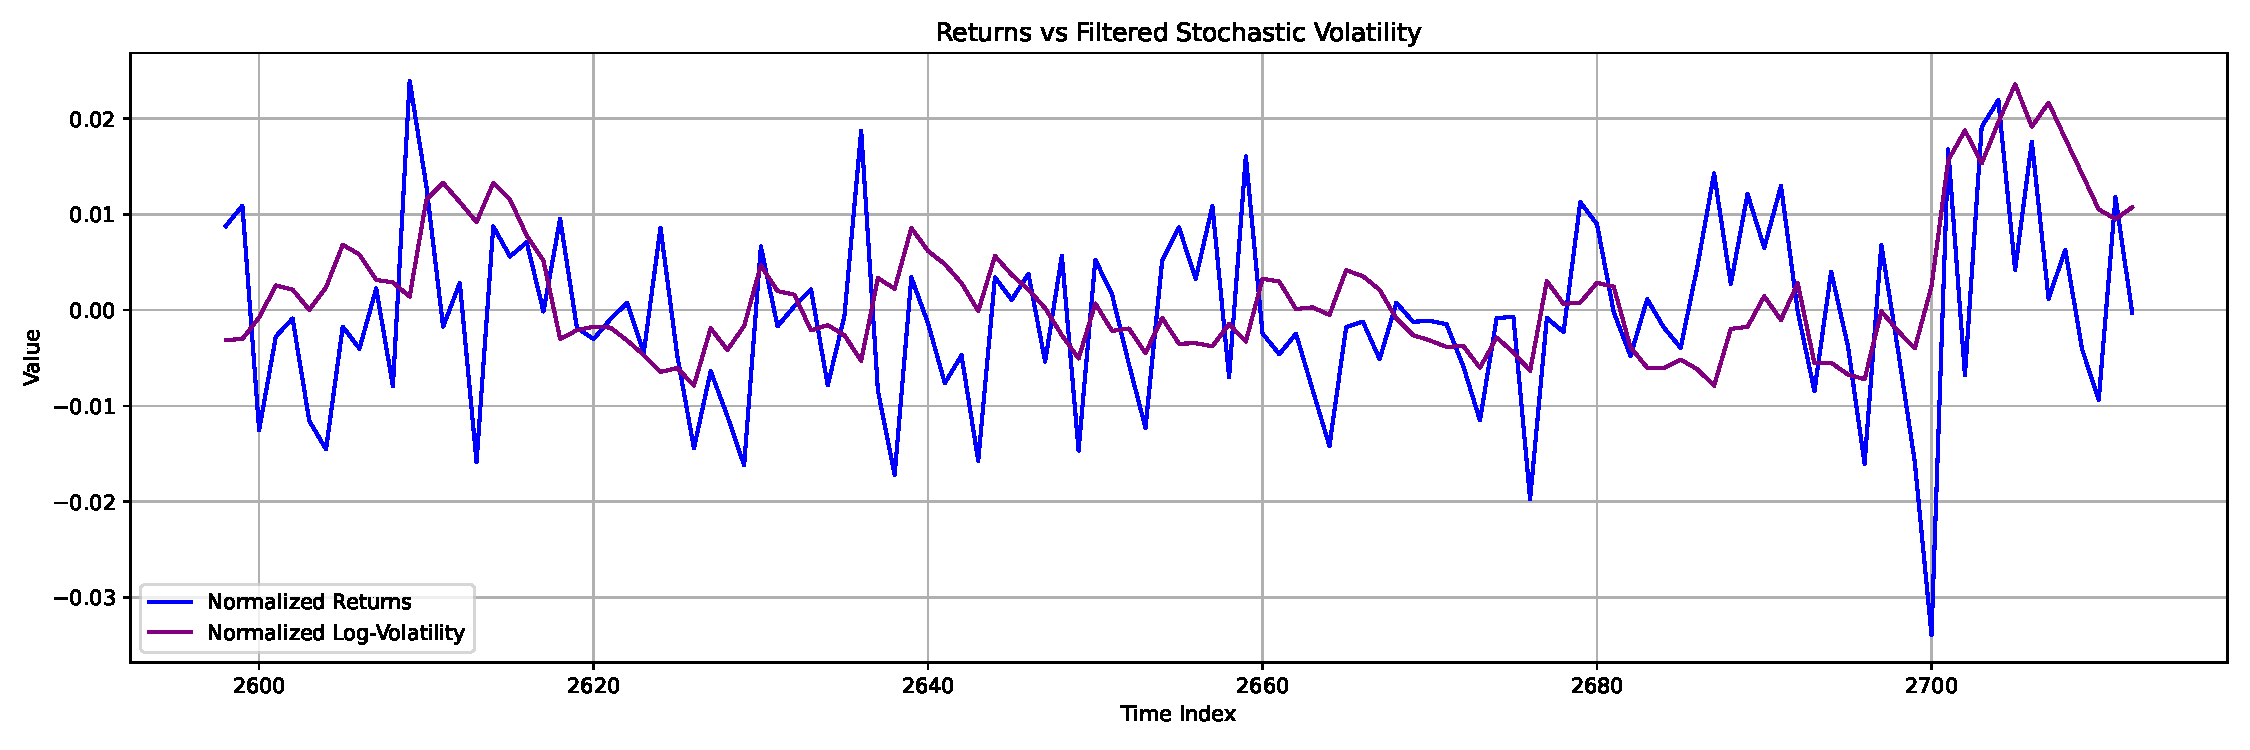
\includegraphics[width=\textwidth]{Images/stochastic_volatility.pdf}
    \caption{Normalized actual returns vs filtered log-volatility (Stochastic Volatility Model).}
    \label{fig:sv_actual_vs_pred}
\end{figure}

\begin{figure}[h!]
    \centering
    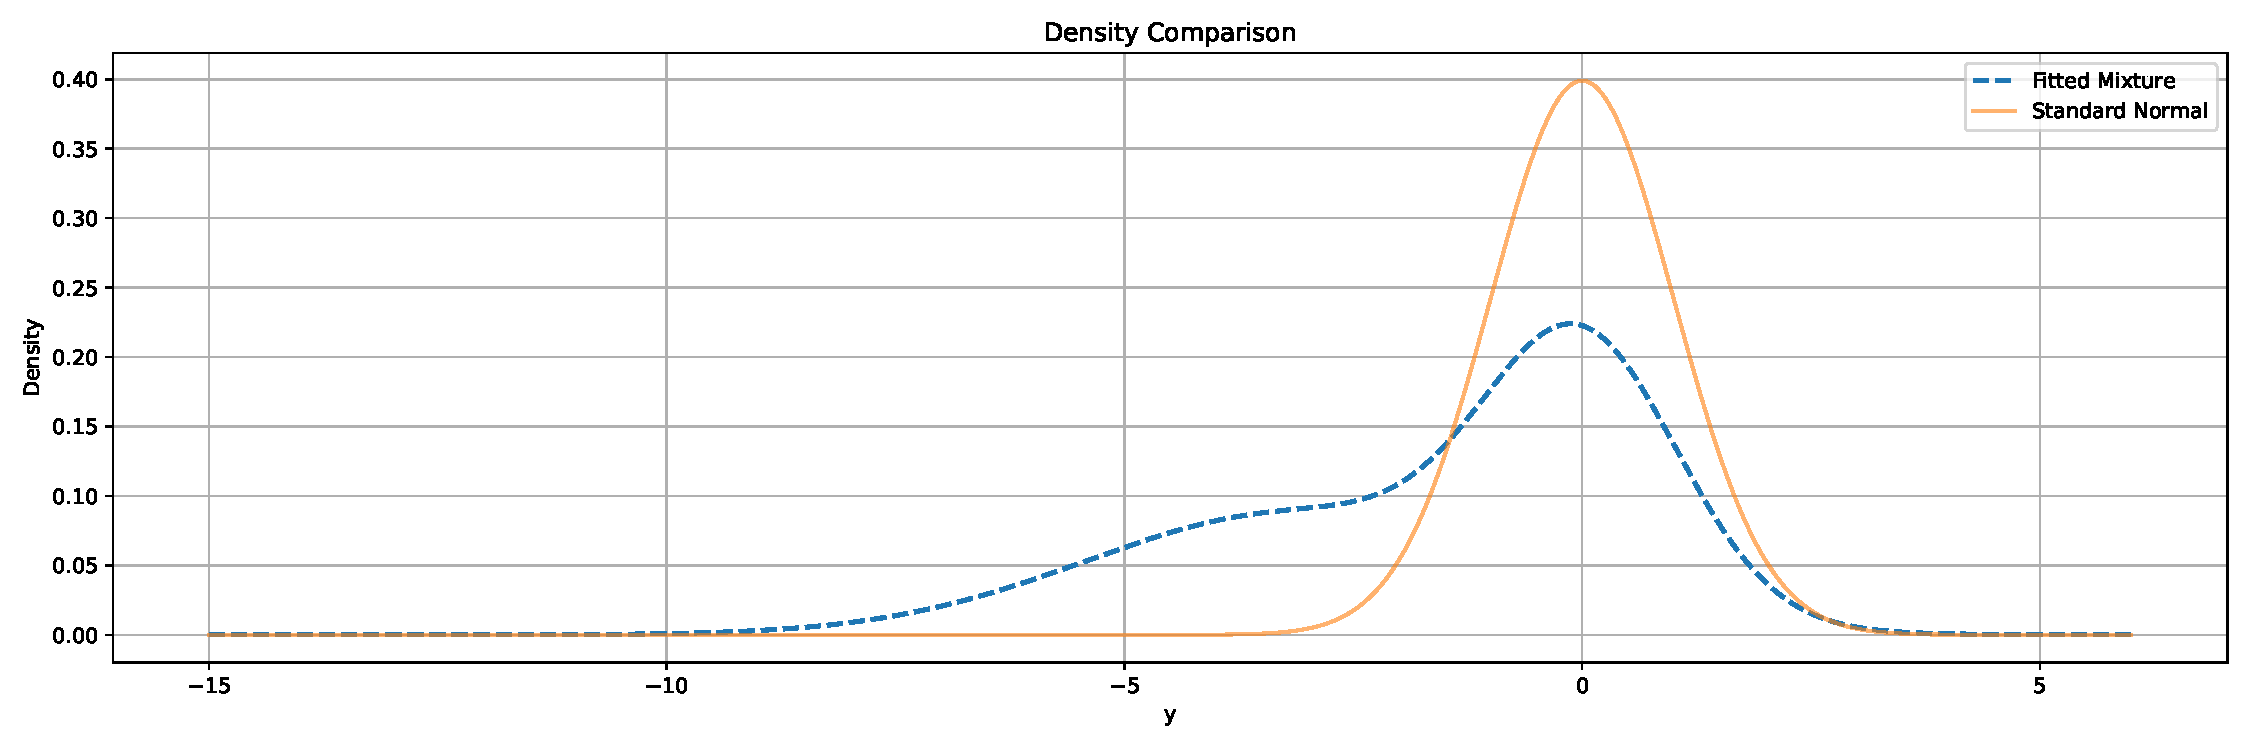
\includegraphics[width=\textwidth]{Images/stochastic_volatility_density.pdf}
    \caption{Density comparison of actual returns vs fitted returns (Stochastic Volatility Model).}
    \label{fig:sv_density}
\end{figure}

\section{Ensemble Learning Results}

\subsection{Actual vs Predicted Returns}
Figure~\ref{fig:ensemble_actual_vs_pred} presents the predicted daily returns from the ensemble meta-learner compared with the actual close returns.

\subsection{Performance Metrics}
\begin{itemize}
    \item \textbf{MetaNet RMSE (Validation):} 0.0065
    \item \textbf{MetaNet RMSE (Test):} 0.0064
    \item \textbf{MetaNet R\textsuperscript{2} Score (Test):} 0.5130
\end{itemize}

\subsection{Base Model Comparison}
Table~\ref{tab:ensemble_base_models} shows the RMSE values for each base model on both the validation and test sets, highlighting the performance of MetaNet as the final predictor.

\begin{table}[h!]
\centering
\caption{RMSE of Base Models and MetaNet (Validation and Test Sets)}
\label{tab:ensemble_base_models}
\begin{tabular}{lcc}
\toprule
\textbf{Model} & \textbf{RMSE (Validation)} & \textbf{RMSE (Test)} \\
\midrule
XGBoost     & 0.00670 & 0.00624 \\
LightGBM    & 0.00670 & 0.00638 \\
CatBoost    & 0.00663 & 0.00636 \\
RandomForest & 0.00667 & 0.00658 \\
ARIMAX      & 0.00713 & 0.00766 \\
MetaNet     & \textbf{0.00655} & \textbf{0.00638} \\
\bottomrule
\end{tabular}
\end{table}

\begin{figure}[h!]
    \centering
    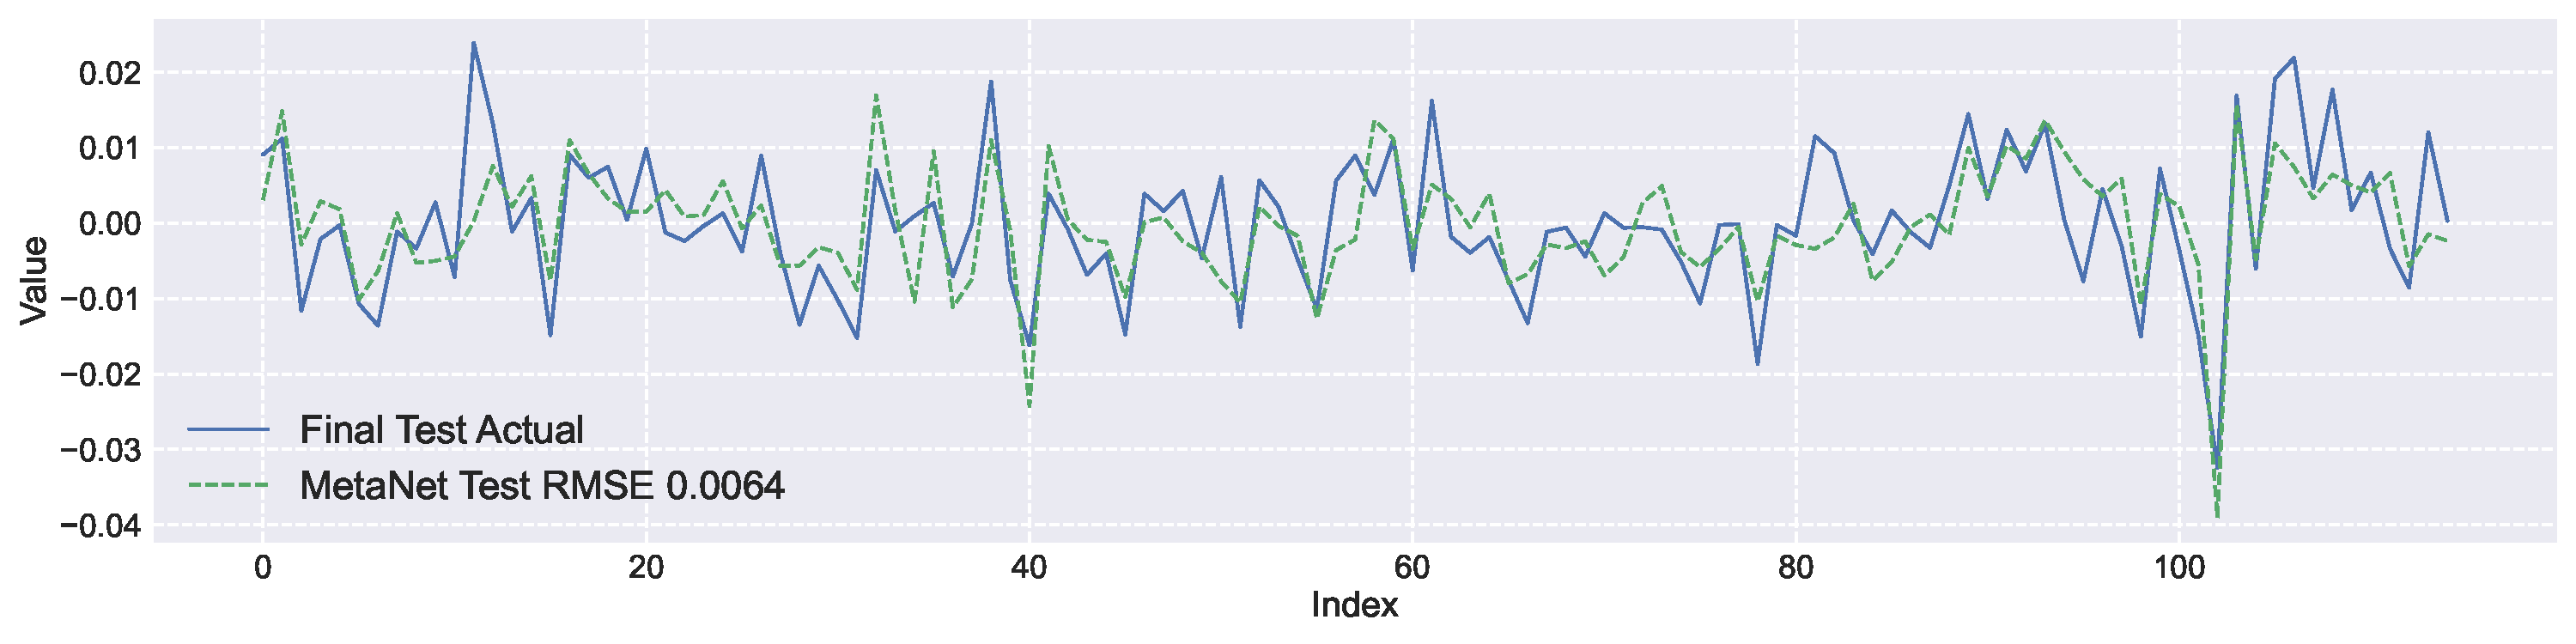
\includegraphics[width=\textwidth]{Images/metanet_final_test_plot__1.pdf}
    \caption{Actual vs Predicted daily close return (Ensemble Meta-Learner).}
    \label{fig:ensemble_actual_vs_pred}
\end{figure}

\section{Transformer GAN Results}
\subsection{Actual vs Predicted Returns}
Figure~\ref{fig:tgan_actual_vs_pred} illustrates the ability of the Transformer-based GAN to replicate daily return dynamics.

\begin{figure}[h!]
    \centering
    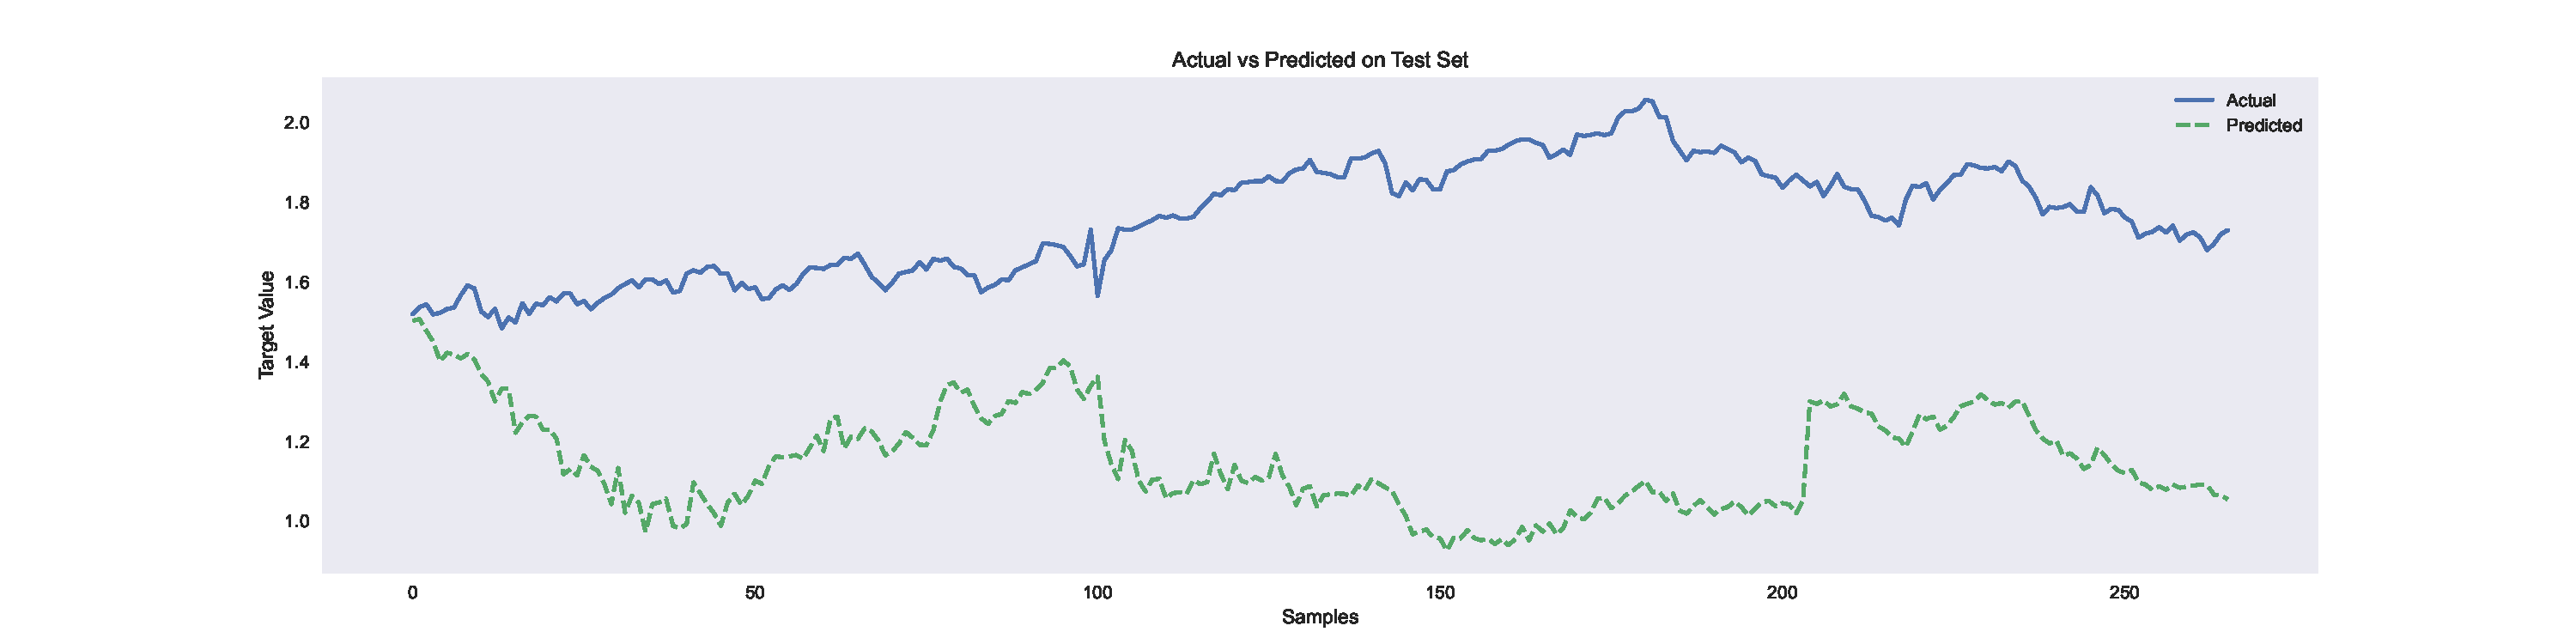
\includegraphics[width=\textwidth]{Images/_8_ActualVsPred_c.pdf}
    \caption{Actual vs Predicted daily close return (Transformer GAN).}
    \label{fig:tgan_actual_vs_pred}
\end{figure}

\noindent After visually inspecting the predicted series, it was observed that the predictions deviate significantly from the actual return values, exhibiting erratic and inconsistent behavior. Due to the highly erroneous nature of these predictions, quantitative performance metrics such as RMSE and R\textsuperscript{2} Score are not reported.

\section{RAGIC Framework Results}
\subsection{Actual vs Predicted Returns}
Figure~\ref{fig:ragic_actual_vs_pred} compares the predicted returns from the RAGIC framework against the actual returns, reflecting the model’s interpretability and precision.

\begin{figure}[h!]
    \centering
    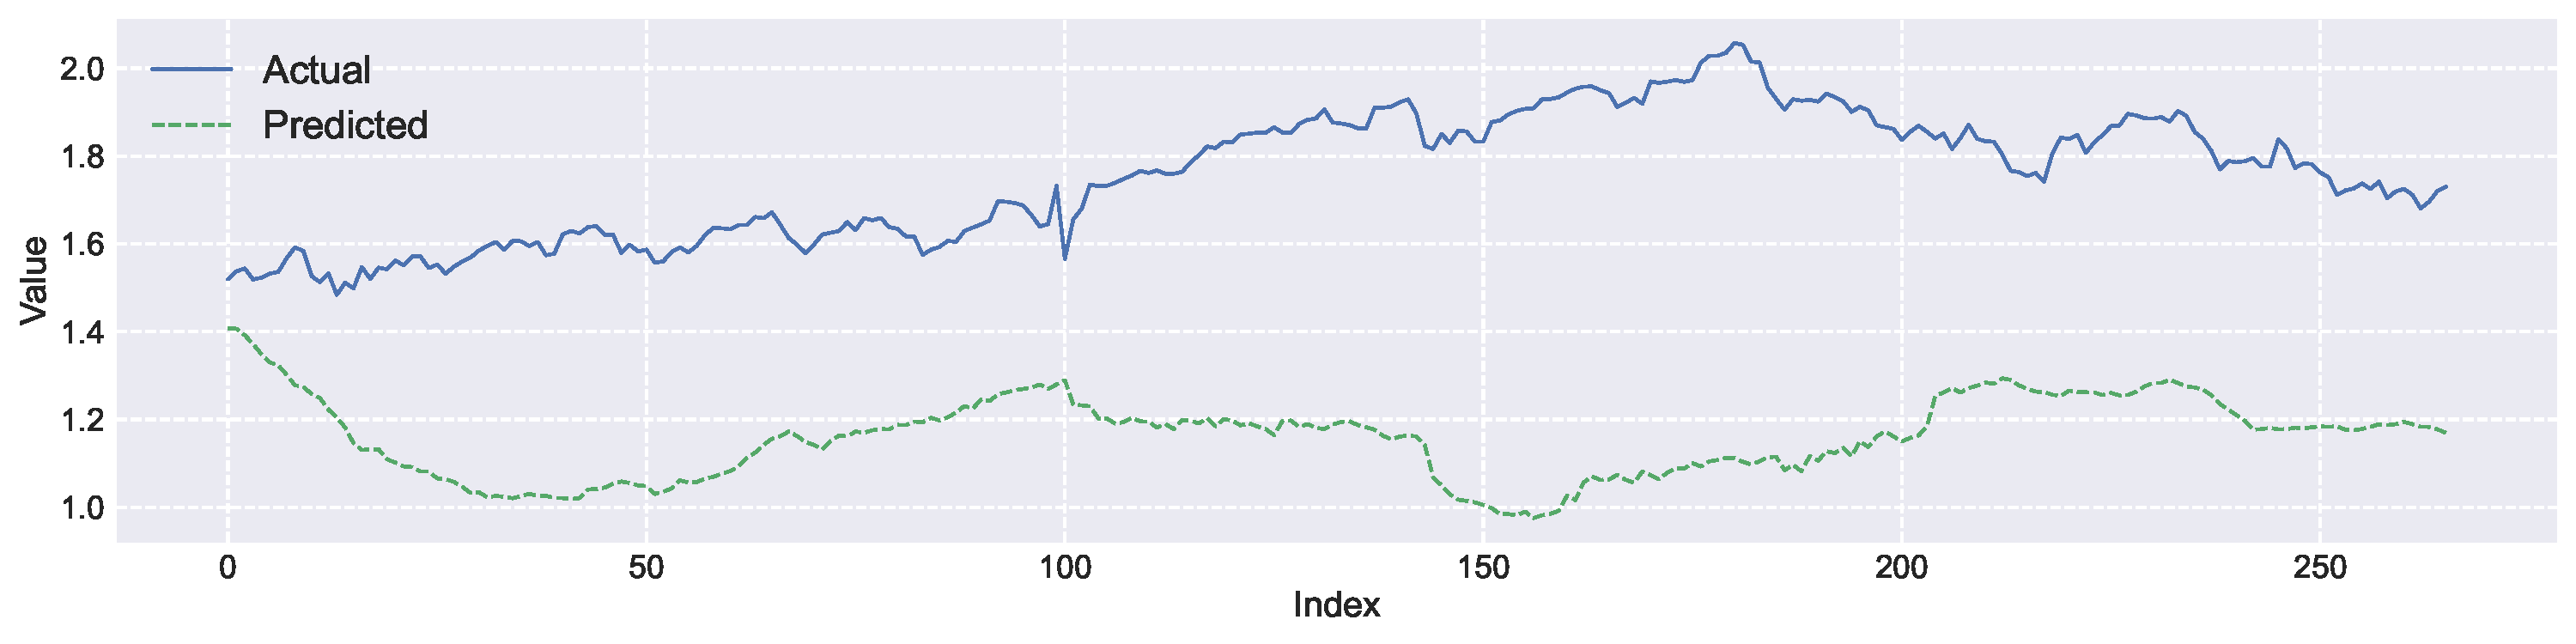
\includegraphics[width=\textwidth]{Images/9_Act_vs_Pred_Point.pdf}
    \caption{Actual vs Predicted daily close return (RAGIC Framework).}
    \label{fig:ragic_actual_vs_pred}
\end{figure}

\noindent Although the RAGIC framework incorporates advanced modules, the predicted returns show significant divergence from the actual values. Based on this visual assessment, RMSE and R\textsuperscript{2} Score are omitted as the model fails to produce stable or meaningful numerical results.

\section{Results Comparison}

\begin{table}[h!]
    \centering
    \caption{Comparison of All Model Performances}
    \label{tab:all_model_comparison}
    \begin{tabular}{|l|c|c|}
    \hline
    \textbf{Model} & \textbf{RMSE} & \textbf{R\textsuperscript{2} Score} \\ \hline
    
    LSTM-RLS (Daily Returns) & 0.76\% & -0.0636 \\ \hline
    LSTM-RLS (Weekly Returns) & 1.44\% & -0.038 \\ \hline
    LSTM-RLS (Daily Close) & 161.8935 & 0.9956 \\ \hline
    LSTM-RLS (Shifted Daily Returns) & 0.24\% & -- \\ \hline
    LSTM-RLS (Multi-Feature Returns) & 0.91\% & -0.061 \\ \hline
    
    DNS - LSTM-SDM & 1082.0187 & 0.8092 \\ \hline
    DNS - LSTM-MA & 688.529 & 0.9227 \\ \hline
    DNS - RBF-SDM & 328.7387 & 0.9823 \\ \hline
    DNS - RBF-MA & 479.8617 & 0.9624 \\ \hline
    
    ARIMAX (Close) & 7431.43 & -35.47 \\ \hline
    ARIMAX (Returns) & 0.703\% & 0.36 \\ \hline
    ARIMAX Model + RLS (Returns) & 0.72\% & 0.32 \\ \hline
    
    Multi-Feature LSTM & -- & -- \\ \hline
    GARCH Model & -- & -- \\ \hline
    Stochastic Volatility Model & 1.04\% & -0.2091 \\ \hline
    Ensemble Learning Model & \textbf{0.638\%} & 0.5130 \\ \hline
    Transformer GAN (TTS GAN) & -- & -- \\ \hline
    RAGIC Architecture & -- & -- \\ \hline
    
    \end{tabular}
\end{table}

\noindent As seen in Table~\ref{tab:all_model_comparison}, the \textbf{Ensemble Learning Model} achieves the lowest RMSE of \textbf{0.638\%}, demonstrating the highest predictive accuracy among all evaluated models. The \textbf{LSTM-RLS (Daily Close)} model also performs exceptionally well with an R\textsuperscript{2} score of 0.9956, highlighting its effectiveness in modeling price levels. In contrast, traditional models like \textbf{ARIMAX (Close)} suffer from high error and a significantly negative R\textsuperscript{2} score. Models with missing metrics such as the \textbf{Multi-Feature LSTM}, \textbf{GARCH Model}, \textbf{Transformer GAN}, and \textbf{RAGIC Architecture} exhibited unstable behavior or extremely poor performance during evaluation, hence their numerical results are omitted. Hybrid models like the \textbf{DNS} and \textbf{LSTM-RLS} variants generally outperform classical approaches, especially in denoised trend and price-based forecasting.
